% -*- latex -*-
%%%%%%%%%%%%%%%%%%%%%%%%%%%%%%%%%%%%%%%%%%%%%%%%%%%%%%%%%%%%%%%%
%%%%%%%%%%%%%%%%%%%%%%%%%%%%%%%%%%%%%%%%%%%%%%%%%%%%%%%%%%%%%%%%
%%%%
%%%% This text file is part of the source of 
%%%% `Introduction to High-Performance Scientific Computing'
%%%% by Victor Eijkhout, copyright 2012/3/4/5
%%%%
%%%% This book is distributed under a Creative Commons Attribution 3.0
%%%% Unported (CC BY 3.0) license and made possible by funding from
%%%% The Saylor Foundation \url{http://www.saylor.org}.
%%%%
%%%%
%%%%%%%%%%%%%%%%%%%%%%%%%%%%%%%%%%%%%%%%%%%%%%%%%%%%%%%%%%%%%%%%
%%%%%%%%%%%%%%%%%%%%%%%%%%%%%%%%%%%%%%%%%%%%%%%%%%%%%%%%%%%%%%%%

Much of the teaching in this book is geared towards enabling you to
write fast code, whether this is through the choice of the right
method, or through optimal coding of a method. Consequently, you
sometimes want to measure just \emph{how fast} your code is. If you
have a simulation that runs for many hours, you'd think just looking
on the clock would be enough measurement. However, as you wonder
whether your code could be faster than it is, you need more detailed
measurements. This tutorial will teach you some ways to measure the
behaviour of your code in more or less detail.

Here we will discuss 
\begin{itemize}
\item timers: ways of measuring the execution time (and sometimes
  other measurements) of a particular piece of code, and
\item profiling tools: ways of measuring how much time each piece of
  code, typically a subroutine, takes during a specific run.
\end{itemize}

\Level 0 {Timers}
\label{sec:perf-timers}

There are various ways of timing your code, but mostly they come down
to calling a routine twice that tells you the clock values:
\begin{verbatim}
  tstart = clockticks()
  ....
  tend = clockticks()
  runtime = (tend-tstart)/ticks_per_sec
\end{verbatim}
For instance, in Fortran there is the \n{system_clock}
routine\index{systemclock@\n{system_clock}}:
\verbatiminput{code/papi/timers/ftimer.F}
with output
\begin{verbatim}
 Clock frequency:       10000
   1.000000       813802544   813826097   2.000000  
\end{verbatim}
In C there is the \n{clock} function:
\verbatiminput{code/papi/timers/ctimer.c}
with output
\begin{verbatim}
clock resolution: 1000000
res: 1.000000e+00
start/stop: 0.000000e+00,2.310000e+00
Time: 2.310000e+00
\end{verbatim}
Do you see a difference between the Fortran and C approaches? Hint:
what happens in both cases when the execution time becomes long? At
what point do you run into trouble?

\Level 1 {System utilities}

There are unix system calls that can be used for timing: \n{getrusage}
and \n{gettimeofday}. These timers have the advantage that they can
distinguish between user time and system time, that is, exclusively
timing program execution or giving \indexterm{wallclock time}
including all system activities.

\Level 0 {Accurate counters}

The timers in the previous section had a resolution of at best a
millisecond, which corresponds to several thousand cycles on a modern
CPU. For more accurate counting it is typically necessary to use
assembly language, such as the Intel \n{RDTSC} (ReaD Time Stamp
Counter)
instruction~\url{http://developer.intel.com/drg/pentiumII/appnotes/RDTSCPM1.HTM}. However,
this approach of using processor-specific timers is not portable. For
this reason, the \indexterm{PAPI} package (\url{http://icl.cs.utk.edu/papi/})
provides a uniform interface to \indexterm{hardware counters}.
You can see this package in action in the codes in
appendix~\ref{app:codes}.

In addition to timing, hardware counters can give you information about 
such things as cache misses and instruction counters. A~processor typically
has only a limited number of counters, but they can be assigned to various tasks.
Additionally, PAPI has the concept of \emph{derived metrics}.

\Level 0 {Profiling tools}

Profiling tools will give you the time spent in various events in the
program, typically functions and subroutines, or parts of the code
that you have declared as such. The tool will then report how many
time the event occurred, total and average time spent, et cetera.

The only tool we mention here is \indexterm{gprof}, the profiler of
the \indexterm{GNU} compiler. The TAU tool, discussed in section~\ref{sec:tau}
for the purposes of tracing,
also has profiling capabilities, presented in a nice graphic way.
Finally, we mention that the \indexterm{PETSc} library
allows you to define your own timers and events.

\begin{verbatim}
% gcc  -g -pg ./srcFile.
% gprof    ./exeFile gmon.out > profile.txt
% gprof -l ./exeFile gmon.out > profile_line.txt
% gprof -A ./exeFile gmon.out > profile_anotated.tx
\end{verbatim}

\Level 1 {MPI profiling}

The MPI library has been designed to make it easy to profile. Each
function such as \n{MPI_Send} does no more than calling
\n{PMPI_Send}. This means that a profiling library can redefine
\n{MPI_Send} to
\begin{itemize}
\item initialize a profiling stage,\item call \n{PMPI_Send}, \item
  finish the profiling stage.
\end{itemize}

\Level 0 {Tracing}

In profiling we are only concerned with aggregate information: how
many times a routine was called, and with what total/average/min/max
runtime. However sometimes we want to know about the exact timing of
events. This is especially relevant in a parallel context when we care
about \indextermbus{load}{unbalance} and \indexterm{idle time}.

Tools such as Vampyr can collect trace information about
events and in particular messages, and render them in displays such as
figure~\ref{fig:vampyr}.
\begin{figure}[ht]
  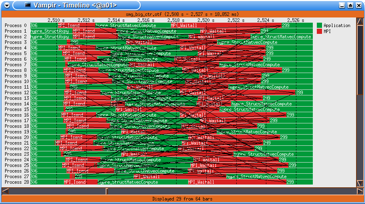
\includegraphics{graphics/vampyrtrace}
  \caption{A Vampyr timeline diagram of a parallel process.}
  \label{fig:vampyr}
\end{figure}

\Level 1 {TAU}
\label{sec:tau}
\index{TAU|(}

The TAU tool~\cite{TAU:ijhpca}
(see \url{http://www.cs.uoregon.edu/research/tau/home.php} for the official documentation)
uses \indexterm{instrumentation} to profile and trace your code. That is, it adds 
profiling and trace calls to your code. You can then inspect
the output after the run.

There are two ways to instrument your code:
\begin{itemize}
\item You can use \indextermsub{dynamic}{instrumentation}, where TAU adds the measurement facility at runtime:
\begin{verbatim}
# original commandline:
% mpicxx wave2d.cpp -o wave2d
# with TAU dynamic instrumentation:
% mpirun -np 12 tau_exec ./wave2d 500 500 3 4 5
\end{verbatim}
\item You can have the instrumentation added at compile time. For
  this, you need to let TAU take over the compilation in some sense.
  \begin{enumerate}
  \item TAU has its own makefiles. The names and locations depend on
    your installation, but typically it will be something like
\begin{verbatim}
export TAU_MAKEFILE=$TAU_HOME/lib/Makefile.tau-mpi-pdt
\end{verbatim}
%% \begin{istc}
%%   At TACC this is taken care of for you:
%% \begin{verbatim}
%% % module load tau
%% % env | grep TAU_MAKEFILE
%% TAU_MAKEFILE=/opt/apps/intel11_1/mvapich2_1_6/tau/2.20.1/x86_64/
%%     lib/Makefile.tau-icpc-papi-mpi-pdt
%% \end{verbatim}
%% \end{istc}
  \item Now you can invoke the TAU compilers \n{tau_cc,sh}, \n{tau_cxx.sh}, \n{tau_f90.sh}.
  \end{enumerate}
\end{itemize}

When you run your program you need to tell TAU what to do:
\begin{verbatim}
export TAU_TRACE=1
export TAU_PROFILE=1
export TRACEDIR=/some/dir
export PROFILEDIR=/some/dir
\end{verbatim}

In order to generate trace plots you need to convert TAU output:
\begin{verbatim}
cd /some/dir # where the trace and profile output went
tau_treemerge.pl
tau2slog2 tau.trc tau.edf -o yourrun.slog2
\end{verbatim}

The \texttt{slog2}\index{slog2 file format} file can be displayed with \indexterm{jumpshot}.

% http://wiki.mpich.org/mpich/index.php/TAU_by_example

\index{TAU|)}
